\documentclass[12pt,a4paper]{report}
\usepackage[utf8]{inputenc}
\usepackage{amsmath}
\usepackage{amsfonts}
\usepackage{amssymb}
\usepackage{graphicx}
\usepackage{caption}
\usepackage{fancyhdr}
\usepackage{titlesec}
\usepackage[top=2in, bottom=0.4in, left=0.6in, right=0.6in]{geometry}
\usepackage{pdfpages}
\usepackage{tabularx}
\usepackage{sidecap}
\usepackage{subcaption}
\usepackage{float}
\usepackage{multirow}


\usepackage[french]{babel}


%Setting header parameters
\addtolength{\voffset}{-72pt}

\pagestyle{fancyplain}
\setlength{\headheight}{50pt}
\lhead{}
\chead{}
\rhead{}

\renewcommand{\headrule}{
	\begin{minipage}{\textwidth}
		\textsl{\footnotesize Rapport de projet informatique} \hfill \textbf{\nouppercase{\leftmark}} \\
		\vspace{-10pt}
		\hrule 
		\vspace{5pt}
		\textsl{\footnotesize Stratification adaptative vs randomized QMC} \hfill 
	\end{minipage}
	\vspace{10pt}
}


\sidecaptionvpos{figure}{c}

\newcommand{\partdiff}[2]{\frac{\partial #1}{\partial #2}}

\renewcommand{\chaptermark}[1]{\markboth{\thechapter.\ #1}{}}
\titleformat{\chapter}[hang]{\bf\huge}{\thechapter}{2pc}{} 
\titlespacing*{\chapter}{0pt}{-30pt}{25pt}

\setlength{\parindent}{0pt}


\newcommand{\R}{\mathbb{R}}
\newcommand{\function}[1]{\texttt{#1}}
\newcommand{\N}{\mathbb{N}}
\newcommand{\esp}[1]{\mathbb{E}\left[ #1 \right]}
\newcommand{\iid}{i.i.d.}
\newcommand{\source}[1]{\emph{#1}}
\newcommand{\class}[1]{\textsc{#1}}


\def \directory {/home/jonathan/Programmation/C++/Projet_C++_S2/Images}

\author{Omar El-Euch, Jonathan Visbecq \\ Stratification adaptative vs randomized QMC}
\title{\centering Master Probabilités et Finance: \\ \textbf{Rapport de projet informatique}}
\begin{document}

\maketitle

\tableofcontents

\chapter{Présentation du sujet}

\section{Sujet}
Le sujet choisi est le suivant:
\begin{center}
\bf
	2.21 Stratification adaptative vs randomized QMC
\end{center}


Comparer les performances des méthodes de stratification exposées dans \cite{EJ08} et de QMC randomisées exposées dans \cite{Tu04} sur les exemples présentés dans \cite{EJ08}.


\section{Présentation mathématique des modèles}

\subsection{Quasi-Monte Carlo randomisé}

\subsection{Stratification adaptative}

\chapter{Tests numériques du code C++}

\section{Quasi-Monte Carlo randomisé}

\subsection{Comparaison des vitesses de convergence}


\begin{figure}[H]
\centering
	\begin{subfigure}[scale=1]{0.45\textwidth}
			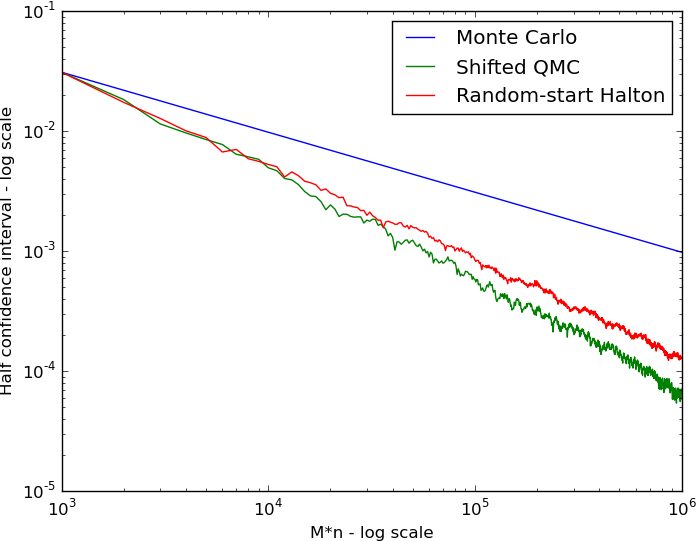
\includegraphics[scale=0.47]{\directory/compare_ciAndTime_MCvsRQMC__CI.png}
			\subcaption{Demi-interval de confiance en fonction du nombre de points générés (échelle 'log-log')}
	\end{subfigure}
	\hfill
	\begin{subfigure}[scale=1]{0.45\textwidth}
		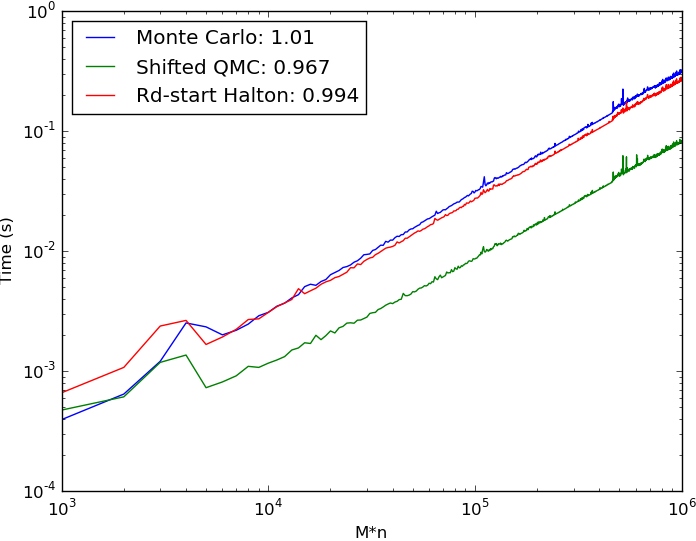
\includegraphics[scale=0.47]{\directory/compare_ciAndTime_MCvsRQMC__time.png}
		\subcaption{Temps (s) de calcul nécessaire en fonction du nombre de points générés (échelle 'log-log')}
	\end{subfigure}
	
\caption{\small Comparaison des temps et vitesses de convergence des méthodes de Monte Carlo randomisées et de Monte Carlo standard pour le calcul de l'intégrale de $f(x_{1},x_{2})=1_{x_{1}<x_{2}}$. M (nombre de pseudo-nombres aléatoires) est fixé à 1000 tandis que N (nombres de quasi-nombres aléatoires) varie de 1 à 1000. Les valeurs indiquées sont les coefficients des pentes (vitesses de convergences).}
\label{fig:rqmc_vitesse_convergence}
\end{figure}

\subsection{Étude du terme de Berry-Essen pour l'intervalle de confiance}
\begin{figure}[H]
\centering
	\begin{subfigure}[scale=1]{0.45\textwidth}
			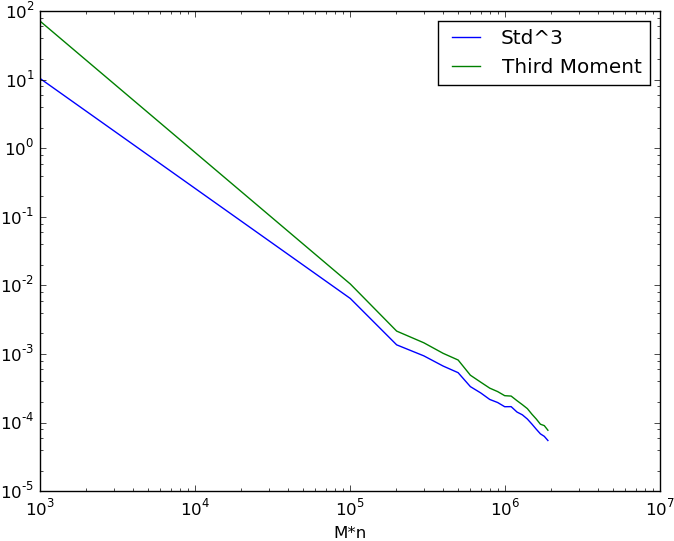
\includegraphics[scale=0.4]{\directory/compare_moments_func1_sqmc.png}
			\subcaption{$\prod_{i=1}^{10} \frac{\pi}{2} \sin(\pi x_{i})$} 
	\end{subfigure}
	\hfill
	\begin{subfigure}[scale=1]{0.45\textwidth}
			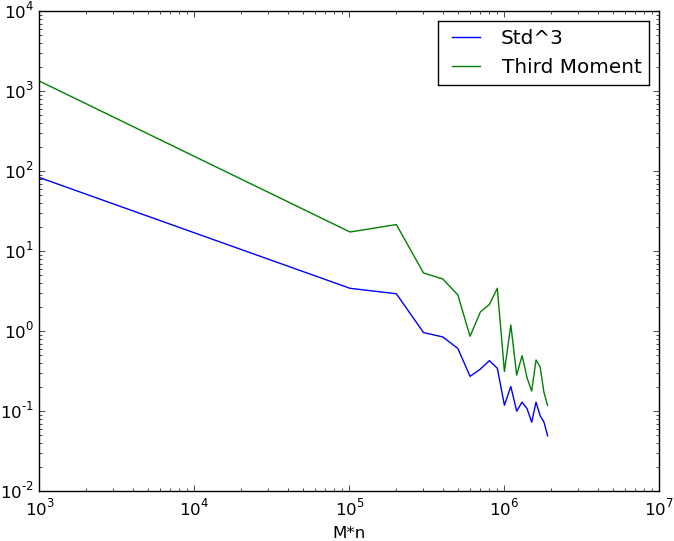
\includegraphics[scale=0.4]{\directory/compare_moments_func2_sqmc.png}
			\subcaption{$\prod_{i=1}^{10} 12(x_{i}-0.5)$} 
	\end{subfigure}
	\vspace{30pt}
	\begin{subfigure}[scale=1]{0.45\textwidth}
			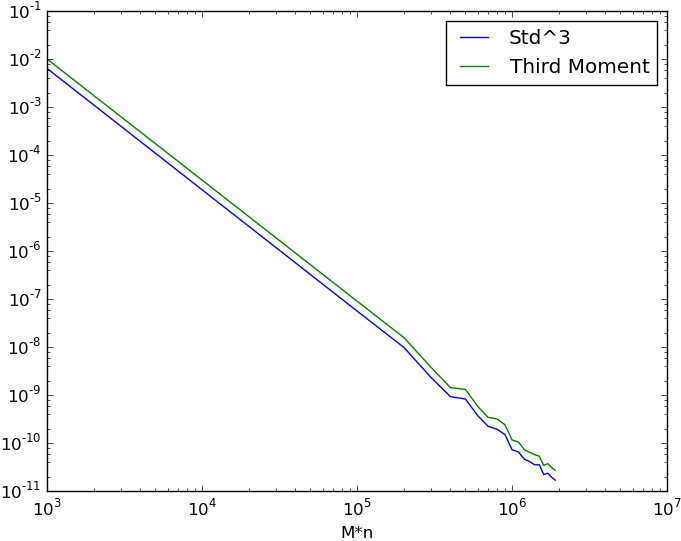
\includegraphics[scale=0.4]{\directory/compare_moments_func3_sqmc.png}
			\subcaption{$\frac{1}{5} \sum_{i=1}^{10} x_{i}$} 
	\end{subfigure}
	\hfill
	\begin{subfigure}[scale=1]{0.45\textwidth}
			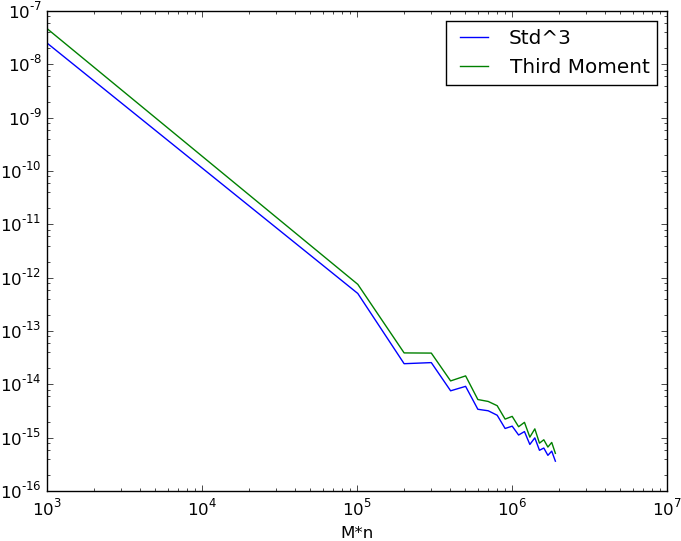
\includegraphics[scale=0.4]{\directory/compare_moments_func4_sqmc.png}
			\subcaption{$\prod_{i=1}^{10} \frac{e^{-|x_{i} - 0.5|}}{2-2e^{0.5}}$} 
	\end{subfigure}
	\vspace{30pt}
	\begin{subfigure}[scale=1]{0.45\textwidth}
			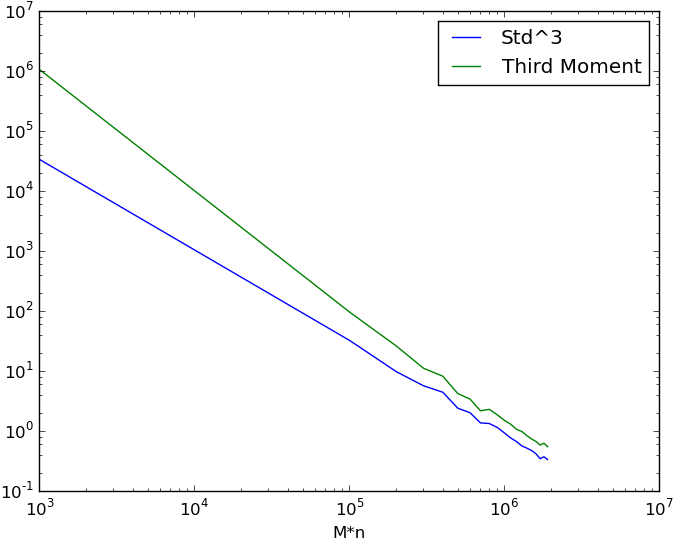
\includegraphics[scale=0.4]{\directory/compare_moments_func5_sqmc.png}
			\subcaption{$\prod_{i=1}^{10} 21_{\{x_{i}>0.5\}}$} 
	\end{subfigure}

	
\caption{\small Comparaison des vitesses de convergence de $\sigma^{3}_{N}$ et de $\beta_{N}$. Comme pour les simulations présentées dans \cite{Tu04}, la vitesse de convergence est sensiblement la même pour toutes les fonctions étudiées.}
\label{fig:rqmc_moments}
\end{figure}


\section{Stratification adaptative}

\subsection{Convergence vers la proportion optimale}

\begin{figure}[H]
\centering
	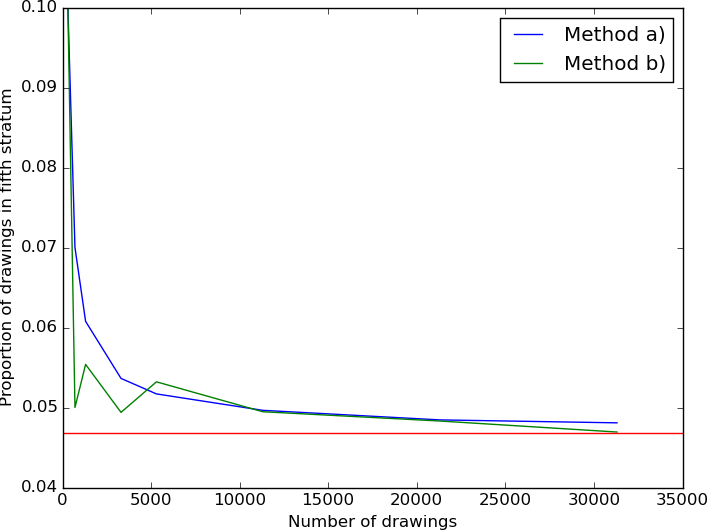
\includegraphics[scale=0.47]{\directory/stratification_reproduce_convergence.png}
	
\caption{\small Convergence de $\frac{N^{k}_{5}}{N^{k}}$ vers la valeur optimale $q_{5}^{*} = 0.04685$ (droite rouge) en fonction de $N^{k}$, pour $k \in [|1,8|]$ et $N^{k}$ prenant les valeurs 300, 700, 1300, 3300, 5300, 11300, 21300, 31300. Les deux méthodes de calcul possible pour la stratification adaptative sont envisagées.}
\label{fig:strat_convergence_proportion}
\end{figure}

\subsection{Comparaison de l'intervalle de confiance estimé à la simulation Monte Carlo}

\begin{figure}[H]
\centering
	\begin{subfigure}[scale=1]{0.45\textwidth}
			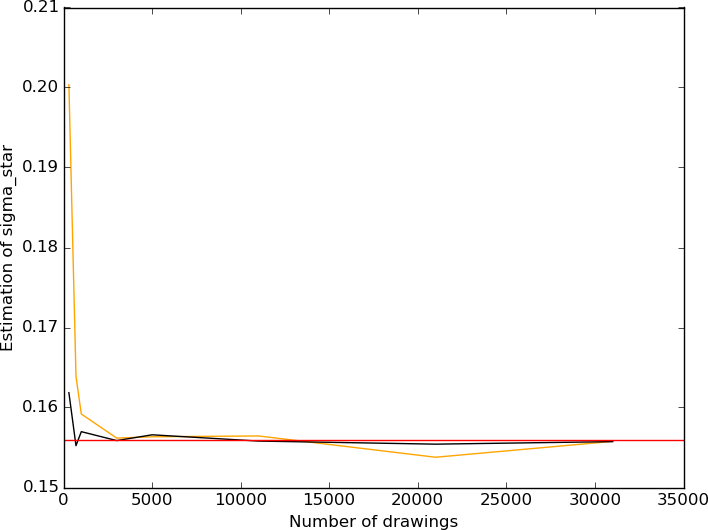
\includegraphics[scale=0.47]{\directory/stratification_reproduce_variance_a.png}
			\subcaption{Méthode a)}
	\end{subfigure}
	\hfill
	\begin{subfigure}[scale=1]{0.45\textwidth}
		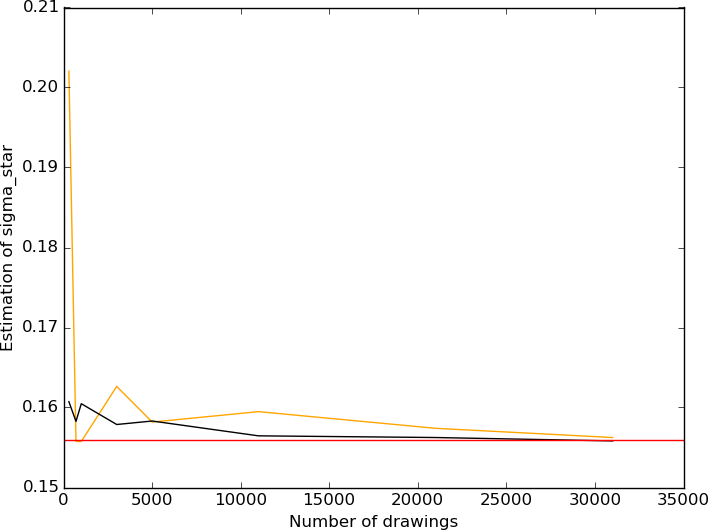
\includegraphics[scale=0.47]{\directory/stratification_reproduce_variance_b.png}
		\subcaption{Méthode b)}
	\end{subfigure}

	
\caption{\small Comparaison entre l'intervalle de confiance estimé à partir de l'estimation de la variance asymptotique $\sigma^{*}$ (en orange) et celui obtenu par simulation Monte Carlo avec 10000 tirages (en noir) pour l'estimation de l'espérance d'une loi normale standard. Les courbes tracées sont estimations de $\sigma^{*}$ (proportionnel à la largeur de intervalle de confiance et la vraie valeur (en rouge)). Avec notre implémentation, la méthode b) semble la moins fiable.}
\label{fig:strat_comparaison_sigma}
\end{figure}

\subsection{Comparaison de la stratification proportionnelle et de la méthode adaptative}

\begin{table}[H]
\centering
	\begin{tabular*}{\textwidth}{@{\extracolsep{\fill}}ccc}
		\hline
		 			    & Stratification proportionnelle 		& Stratification adaptative \\ 
		 			    																	\\
		\hline
		Variance	    & 1.26e-06		                        & 7.82e-07	                \\
		Temps (s)      	& 0.0249		                        & 0.0256                    \\
		Variance*temps	& 3.14e-08                              & 2.00e-08		            \\
		\hline
	\end{tabular*}
\caption{Comparaison des résultats entre les méthodes d'allocation proportionnelles et adaptative pour l'estimation de l'espérance d'une loi normale standard. Nous utilisons 31300 tirages pour la stratification, répartie successivement en 300, 1300, 11300 puis 31300 tirages pour la méthode adaptative. L'expérience est répétée 10000 fois et les valeurs présentées sont les moyennes des résultats obtenus.}
\label{tab:strat_comparaison_proportionnelle_adaptative}
\end{table}

\subsection{Comparaison avec les résultats de \cite{EJ08} pour les options asiatiques}



\begin{figure}[H]
\centering
	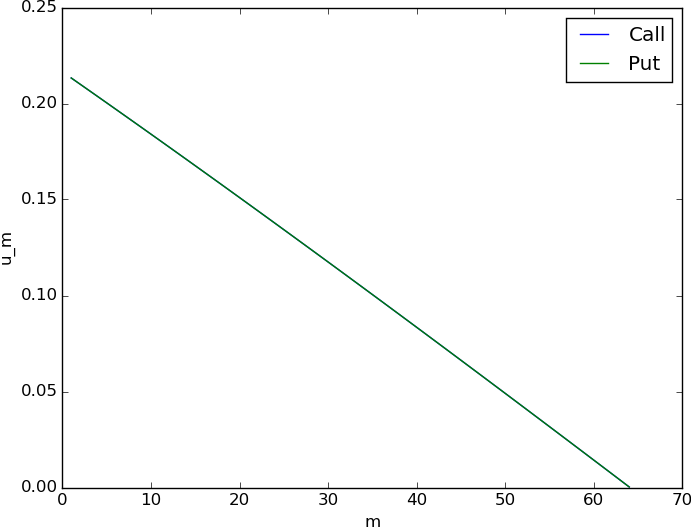
\includegraphics[scale=0.47]{\directory/stratification_asian_u.png}

\caption{\small Composantes $u_{m}$ du vecteur unitaire $u$ donnant la direction de stratification en fonction de $m$ pour le call et le put asiatique. Paramètres: d=64, K=45.}
\label{fig:strat_u}
\end{figure}


\begin{figure}
\centering
	\begin{subfigure}[scale=1]{0.45\textwidth}
			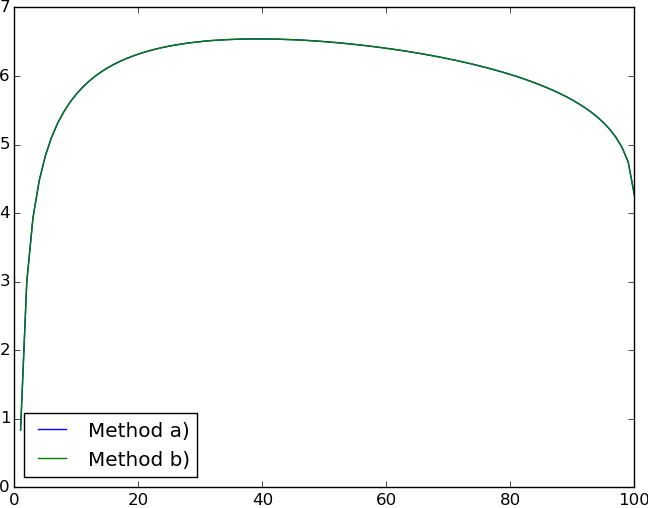
\includegraphics[scale=0.47]{\directory/../Images/stratification_asian_call_means.png}
			\subcaption{Estimation de $\esp{f\left( X_{i} \right)}$.}
	\end{subfigure}
	\hfill
	\begin{subfigure}[scale=1]{0.45\textwidth}
		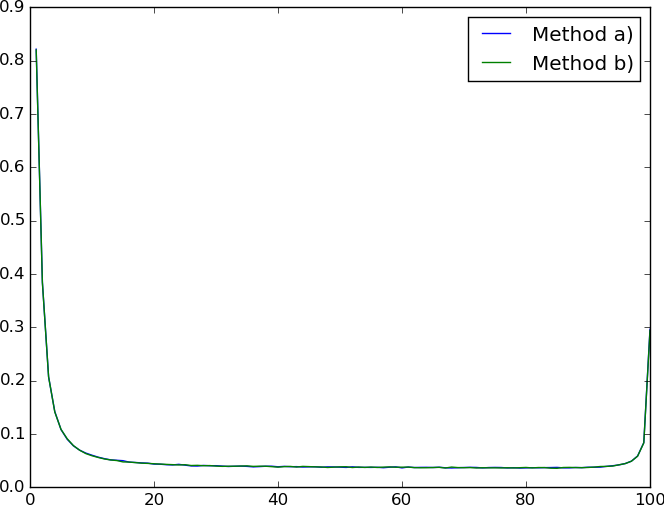
\includegraphics[scale=0.47]{../Images/stratification_asian_call_stds}
		\subcaption{Estimation de $\sigma_{i}$.}
	\end{subfigure}
\caption{Estimation de $\esp{f\left( X_{i}] \right)}$ et de $\sigma_{i}$ sur chaque strate en fonction de i pour le call asiatique. Paramètres: $d=64$ et $K=45$.}
\label{fig:stratification_asian_call_means_stds}
\end{figure}
\begin{figure}
\centering
	\begin{subfigure}[scale=1]{0.45\textwidth}
			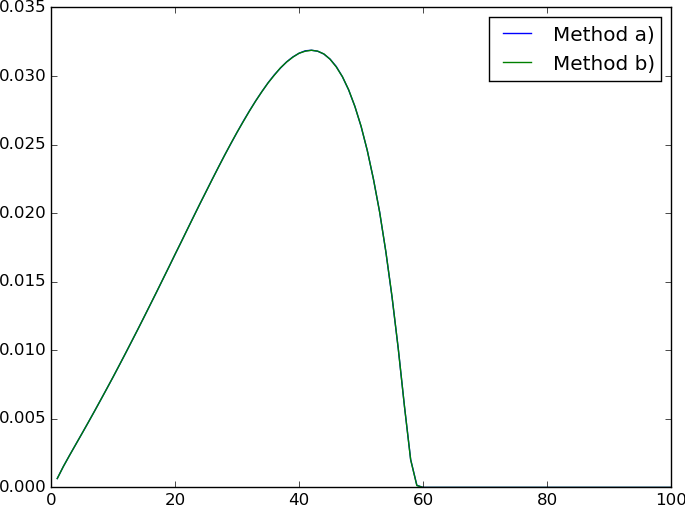
\includegraphics[scale=0.47]{\directory/../Images/stratification_asian_put_means.png}
			\subcaption{Estimation de $\esp{f\left( X_{i} \right)}$.}
	\end{subfigure}
	\hfill
	\begin{subfigure}[scale=1]{0.45\textwidth}
		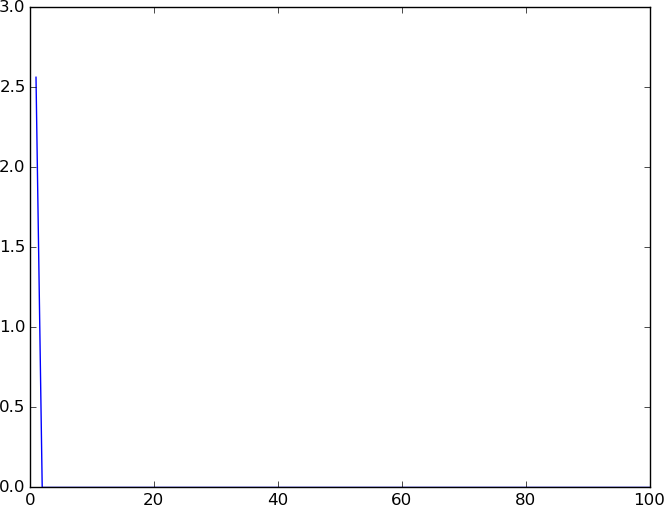
\includegraphics[scale=0.47]{../Images/stratification_asian_put_stds}
		\subcaption{Estimation de $\sigma_{i}$.}
	\end{subfigure}t
\caption{Estimation de $\esp{f\left( X_{i}] \right)}$ et de $\sigma_{i}$ sur chaque strate en fonction de i pour le put asiatique. Paramètres: $d=64$ et $K=45$.}
\label{fig:stratification_asian_put_means_stds}
\end{figure}





\begin{table}[H]
\centering
	\begin{tabular*}{\textwidth}{@{\extracolsep{\fill}}ccccccc}
		\hline
			                &   &   & \multicolumn{2}{|c|}{Variance} &                      \\ 
		\hline
		
		d	                & K  & Price  & Adap.    & Prop.    & Ratio Prop. / Adap        \\
		\hline
		\multirow{3}{*}{16} & 45 & 6.05   & 2.63e-08 & 1.08e-07 & 4.11	                    \\
							& 50 & 1.91   & 1.20e-07 & 7.76e-06 & 64.69	                    \\
							& 55 & 0.20   & 5.29e-09 & 4.33e-07 & 81.74	                    \\
	 \hline
		\multirow{3}{*}{64} & 45 & 6.00   & 3.53e-09 & 2.32e-08 & 6.58	                    \\
							& 50 & 1.84   & 1.00e-09 & 3.05e-09 & 3.04                      \\
							& 55 & 0.17   & 6.55e-09 & 7.36e-07 & 112.35	                \\
		\hline
	\end{tabular*}
\caption{Comparaison des allocations proportionnelles et adaptative pour l'exemple du call asiatique. Les ratios trouvés sont environ 2 fois supérieures à ceux de \cite{EJ08}.}
\label{tab:strat_asian_call}
\end{table}

\begin{table}[H]
\centering
	\begin{tabular*}{\textwidth}{@{\extracolsep{\fill}}ccccccc}
		\hline
			                &   &   & \multicolumn{2}{|c|}{Variance} &                      \\ 
		\hline
		
		d	                & K  & Price  & Adap.    & Prop.    & Ratio Prop. / Adap        \\
		\hline
		\multirow{3}{*}{16} & 45 &    &  &  & 	                    \\
							& 50 &    &  &  & 	                    \\
							& 55 &    &  &  & 	                    \\
		\hline
		\multirow{3}{*}{64} & 45 &    &  &  & 	                    \\
							& 50 &    &  &  &                       \\
							& 55 &    &  &  & 	                \\
		\hline
	\end{tabular*}
\caption{Comparaison des allocations proportionnelles et adaptative pour l'exemple du put asiatique avec $S0 = 50$, $r = 0.05$, $\sigma = 0.1$, $T = 1.$ et 100 strates. 1000000 de tirages sont utilisés, répartie progressivement en 100000, 400000, 500000 et 1000000 pour la méthode adaptative.}
\label{tab:strat_asian_put}
\end{table}


\chapter[Comparaison sur les exemples de \cite{EJ08}]{Comparaison des deux méthodes de réduction de variance sur les exemples de \cite{EJ08}}

\subsection{Loi normale standard}

\begin{figure}[H]
\centering
	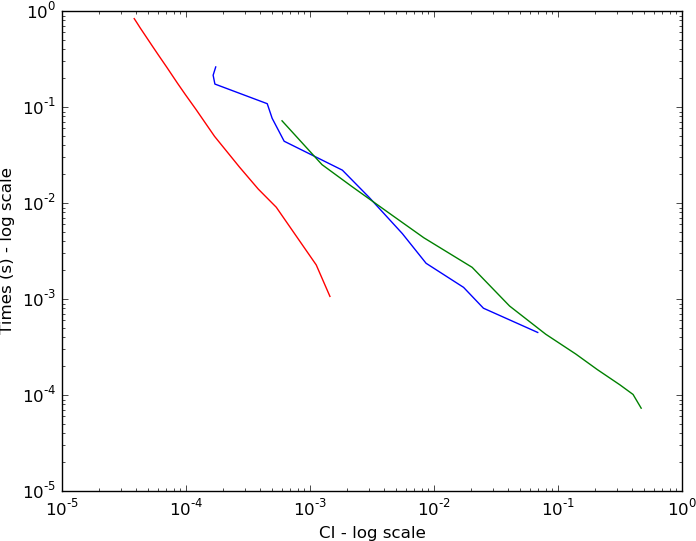
\includegraphics[scale=0.47]{\directory/compare_gaussian.png}

\caption{\small Etude des vitesses de convergence entre les trois méthodes de réduction de variance: stratification adaptative (en rouge), Shifted SQRT (en bleu) et Random-start Halton (en vert) pour l'example de la gaussienne standard. Les valeurs indiquées sont les pentes des droites (vitesses de convergence).}
\label{fig:compare_gaussian}
\end{figure}


\subsection{Options asiatiques}

\begin{figure}[H]
\centering
	\begin{subfigure}[scale=1]{0.45\textwidth}
			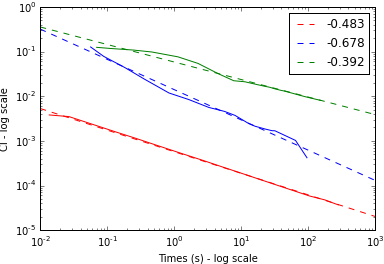
\includegraphics[scale=0.47]{\directory/compare_asian_64_45.png}
			\subcaption{$d=64$ et $K=45$} 
	\end{subfigure}
	\hfill
	\begin{subfigure}[scale=1]{0.45\textwidth}
			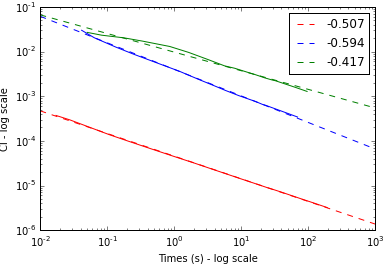
\includegraphics[scale=0.47]{\directory/compare_asian_64_55.png}
			\subcaption{$d=64$ et $K=45$} 
	\end{subfigure}
	\vspace{30pt}
	\begin{subfigure}[scale=1]{0.45\textwidth}
			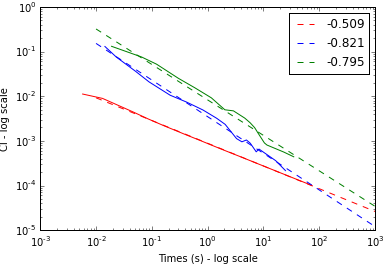
\includegraphics[scale=0.47]{\directory/compare_asian_16_45.png}
			\subcaption{$d=64$ et $K=45$} 
	\end{subfigure}
	\hfill
	\begin{subfigure}[scale=1]{0.45\textwidth}
			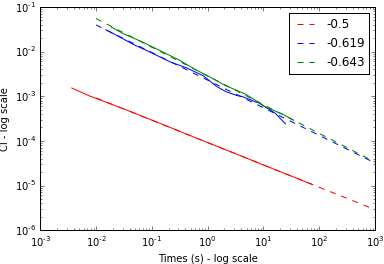
\includegraphics[scale=0.47]{\directory/compare_asian_16_55.png}
			\subcaption{$d=64$ et $K=45$} 
	\end{subfigure}
	
\caption{\small Etude des vitesses de convergence entre les trois méthodes de réduction de variance: stratification adaptative (en rouge), Shifted SQRT (en bleu) et Random-start Halton (en vert) pour l'example du call asiatique. Les lignes en pointillés sont les droites de régression, dont les pentes sont indiquées en légende.}
\label{fig:compare_asian_call}
\end{figure}

\chapter{Présentation du code C++}

L'intégrité du code informatique est écrit en C++11. Le type de programmation employée est générique, afin de faciliter l'écriture des tests et scripts.\\



Le code se compose notamment de:

\begin{itemize}
	\item Alias \class{array$<$dim$>$} et fonctions template du fichier \source{my\_array.hpp} pour simuler les opérations basiques d'algèbre linéaire sans avoir à faire appel à une librairie externe. \\
	
	\item Des classes représentant des générateurs (\source{generator.hpp}) de nombres pseudo-aléatoires ou quasi-aléatoires respectant les caractéristiques suivantes:
	\begin{itemize}
		\item[\Huge\textbf{.}] argument template \textit{unsigned dim} représentant la dimension des points à générer.
		\item[\Huge\textbf{.}] surcharge de l'opérateur () sans arguments renvoyant un \textit{Array$<$dim$>$}.\\
	\end{itemize}
	
	Les générateurs présents sont les suivants:
	\begin{itemize}
		\item[.] \class{uniform\_gen} (\source{uniform\_generator.hpp}) qui appel une fonction externe dont un champ statique contient un générateur MT19937 de la librairie standard. Ainsi, toutes les instance de cette classes représenteront des variable aléatoires uniforme indépendantes.
		\item[.] \class{uniform\_gen\_fixed} (\source{uniform\_generator.hpp}) qui utilise un générateur MT19937 différent pour chaque instance mais de seed identique.
		\item[.] \class{kakutani} (\source{kakutani.hpp}) représentant une suite de Kakutani.
		\item[.] \class{halton} (\source{kakutani.hpp}) représentant une suite de Halton comme classe dérivée d'une suite de Kakutani.
		\item[.] \class{halton\_fast} (\source{kakutani.hpp}) représentant une suite de Halton, mais pour laquelle la génération des points est plus rapide qu'avec l'addition de nombre p-adique vue en cours. La méthode est inspirée de ...
		\item[.] \class{faure} (\source{faure.hpp}) représentant une suite de Faure.
		\item[.] \class{tore} (\source{tore.hpp}) représentant une suite générée par rotation ... 
		\item[.] \class{sqrt} (\source{tore.hpp}) représentant ...\\
	\end{itemize}
	
	\item Des distributions (\source{distribution.hpp}), permettant de calculer des réalisations de variables aléatoires à partir des points générés par un générateur. Les distribution respectent les caractéristique suivantes:
	\begin{itemize}
		\item[\Huge\textbf{.}] typedef \textit{result\_type} pour le type de retour de la distribution
		\item[\Huge\textbf{.}] attribut \textit{static constexpr unsigned dim\_alea} pour la dimension des points nécessaires au calcul des réalisations
		\item[\Huge\textbf{.}] surcharge de l'opérateur () prenant en argument un \textit{const Array$<$dim$>$\&} et renvoyant un objet de type \textit{result\_type}\\
	\end{itemize}
	
	Les distributions présentes sont les suivantes:
	\begin{itemize}
		\item[.] \class{uniform} (\source{uniform.hpp}) pour les variables aléatoires uniformes sur un intervalle de $\R$
		\item[.] \class{gaussian\_ind}$<$unsigned dim$>$ (\source{gaussian\_ind.hpp}) pour les variables aléatoires gaussiennes multidimensionnelles dont toutes les composantes sont mutuellement indépendantes. On utilise la méthode de Box-Müller pour être compatible avec les générateurs QMC.
		\item[.] \class{stdbrownian}$<$unsigned t\_dim$>$ (\source{process.hpp}) pour les mouvements Browniens (le type de retour est un alias sur un tableau de pairs (temps,valeur)). Le template repsésente le nombre de temps du processus.
		\item[.] \class{black\_scholes}$<$unsigned t\_dim$>$ pour les processus de Black-Scholes (\source{process.hpp}).
		\item[.] \class{Normal\_Interval}$<$unsigned dim$>$ (\source{normal\_interval.hpp})pour les variable aléatoires gaussiennes multidimensionnelles standards conditionnellement à ce que leur projection sur un axe soit dans un intervalle donné (pour les méthodes de stratification). On utilise ici une approximation de l'inverse de la fonction de répartition par la méthode de Beasley-Springer-Moro [Glasserman 2004].
		\item[.] \class{composed\_dist}$<$typename Dist$>$ permettant de composer une distribution avec une fonction.\\
	\end{itemize}
	
	\item Sont également implémentés comme des distributions les méthodes de Monte Carlo randomisées (pour pouvoir les passer à un objet \class{monte\_carlo}, voire ci-après):
	\begin{itemize}
		\item[.] \class{shifted\_qmc}$<$typename Dist, typename QMC\_Generator$>$ (\source{shifted\_qmc.hpp}) pour les méthodes de quasi-Monte Carlo translatées.
		\item[.] \class{randstart\_halton}$<$typename Dist$>$ (\source{random\_start\_halton.hpp}) pour la méthode de Halton à point initial aléatoire.\\
	\end{itemize}
	
	\item \class{rand\_var} (\source{rand\_var.hpp})$<$typename Dist, typename Generator$>$ permet d'associer un générateur à une distribution.\\
	
	\item \class{monte\_carlo}$<$typename Dist$>$ pour les simulations Monte Carlo. Le choix adopté est d'avoir la distribution en argument template et de passer à chaque appel le générateur à utiliser et le nombre de réalisations, afin de faciliter les comparaisons entre plusieurs générateurs.\\
	
	\item \class{stratification}$<$template $<$unsigned$>$ Dist\_Strat, unsigned dim, nb\_strats$>$ (\source{stratification.hpp}) implémentant la méthode de stratification standard pour l'évaluation de fonctionnelles de la distribution Dist\_Strat<dim> en dimension dim, avec nb\_strats strates. A l'instanciation, la fonctionnelle, les bornes des strates, la direction de stratification et les probabilités des strates sont précisées. L'appel à l'algorithme nécessite un générateur, le nombre de réalisation et les allocations sur chaque strate (dont l'omission conduit à l'algorithme proportionnel).\\
	
	\item  \class{adaptive\_stratification}$<$template $<$unsigned$>$ Dist\_Strat, unsigned dim, nb\_strats$>$ (\source{adaptive\_stratification.hpp}) pour l'algorithme de stratification adaptative de \cite{EJ08}. Les paramètres d'instanciation sont les mêmes que précédemment, plus le choix de la méthode ( a) ou b) ). La première de l'appeler est de fournir le générateur, et un tableau contenant les nombres successifs de réalisations à chaque itération. Une seconde fonction d'appel permet de réaliser un itération à la fois affin de raffiner. Cela permet d'avoir accès à l'état de l'algorithme itération par itération.\\
	
	\item \class{p\_adic} (\source{p\_adic.hpp, p\_adic.cpp}) permet de représenter et de manipuler les nombres p-adiques.\\
\end{itemize}

Le fichier \source{payoff.hpp} contient notamment les fonctions de payoff des options asiatiques nécessaires pour le deuxième exemple de \cite{EJ08}.\\

Enfin, le \source{scripts.hpp} et \source{scripts.cpp} contiennent les fonctions effectuant les simulations et tests et sont lancés depuis le \source{main.cpp}.




\bibliography{bibliographie}{}
\bibliographystyle{alpha}
\end{document}